\documentclass[10pt, pdf, hyperref={unicode}]{beamer}
\usepackage[T2A]{fontenc}
\usepackage[utf8]{inputenc}
\usepackage[english, russian]{babel}
\usepackage{amssymb, amsfonts, amsmath, amsthm, microtype, pdfpages}

\usetheme{Madrid}
\usecolortheme{beaver}

\title{<<Математическая модель импульсного погружателя, оптимального по коэффициенту асимметрии>>}
\date{10.06.2019}
\author{Уткин Артем Александрович}

\setbeamertemplate{frametitle}[default][center]
\setbeamertemplate{navigation symbols}{}
\setbeamertemplate{footline}[page number]


\begin{document}

    \begin{frame} % титульный лист 
        \titlepage
        \begin{center}
            Бакалаврская работа\\
            Направление 01.03.04 Прикладная математика\\
            Профиль Применение математических методов к решению инженерных и экономических задач
        \end{center}
    \end{frame}


    \begin{frame}
        \frametitle{Актуальность проблемы}
        \begin{center}
            \begin{minipage}[h]{0.97\linewidth}
                \begin{minipage}[h]{0.95\linewidth}
                    На сегодняшний день в строительной сфере довольно часто возникает потребность в вибропогружателях для погружения свайных элементов в землю.
                    \newline
                    Такая востребованность порождает задачу оптимизации характеристик вибропогружателей для получения наилучшего результата их работы.
                    \newline
                    Решение задачи прикладными методами несомненно актуальна в данный момент и соответствует профилю.
                \end{minipage}
                \begin{minipage}[h]{0.25\linewidth}
                    \begin{figure}[h]
                        \centering
                        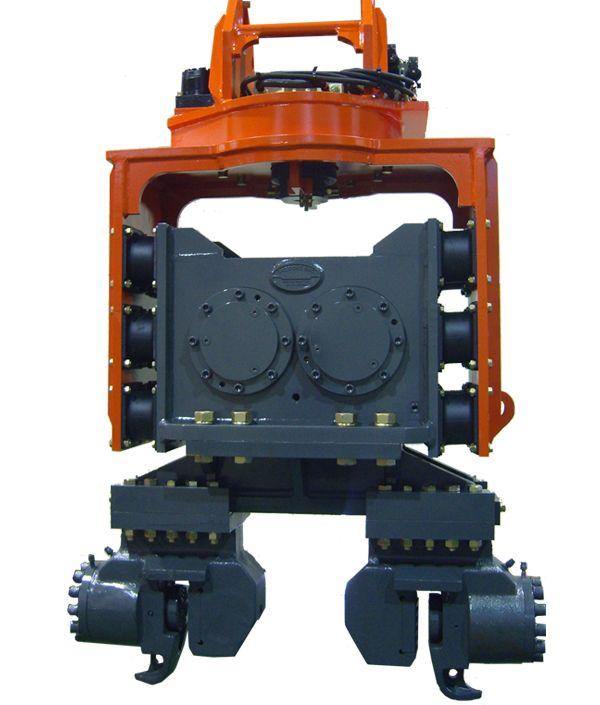
\includegraphics[width=1\linewidth]{../img/photo_1.jpg}
                    \end{figure}
                \end{minipage}
                \hfill
                \begin{minipage}[h]{0.25\linewidth}
                    \begin{figure}[h]
                        \centering
                        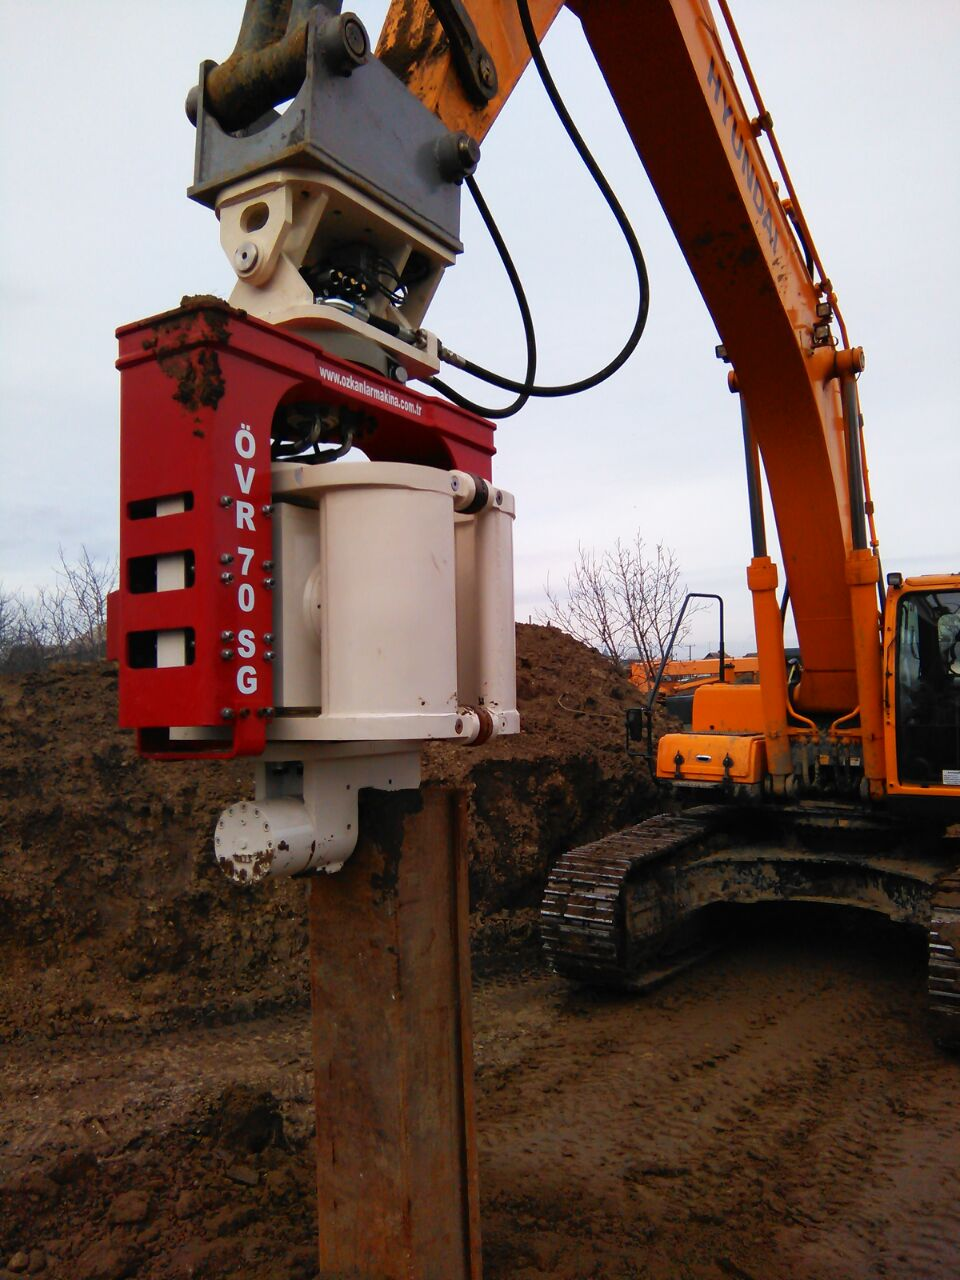
\includegraphics[width=1\linewidth]{../img/photo_2.jpg}
                    \end{figure}
                \end{minipage}
                \hfill
                \begin{minipage}[h]{0.32\linewidth}
                    \begin{figure}[h]
                        \centering
                        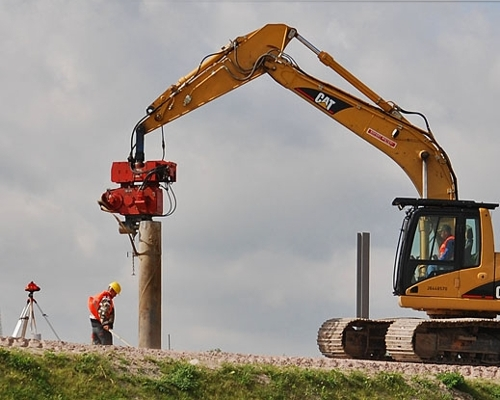
\includegraphics[width=1\linewidth]{../img/photo_3.jpg}
                    \end{figure}
                \end{minipage}
            \end{minipage}
        \end{center}
    \end{frame}


    \begin{frame}
        \frametitle{Постановка задачи}
        \begin{center}
            \begin{minipage}[h]{0.97\linewidth}
                Для решения такой задачи необходимо на основе теории вибрационных машин и теоремы об оптимальности импульса Максвелла-Фейера
                разработать ПО для автоматизированного расчета характеристик импульсного погружателя
                с возможностью ввода начальных данных и наглядного вывода результатов.
            \end{minipage}
        \end{center}
    \end{frame}


    \begin{frame}
        \frametitle{Конструкция вибропогружателя}
        \begin{center}
            \begin{minipage}[h]{0.97\linewidth}
                \begin{minipage}[h]{0.5\linewidth}
                    Принцип действия погружателя основан на эффекте резкого снижения сопротивлению погружения свайного элемента
                    при сообщении последнему вибрации.\\
                    При вращении дебалансов на их ось крепления действует центробежная сила и вибрационный погружатель получает вибрирующее движение,
                    которое сообщается свайному элементу через наголовник.
                \end{minipage}
                \hfill
                \begin{minipage}[h]{0.36\linewidth}
                    \begin{figure}[h]
                        \centering
                        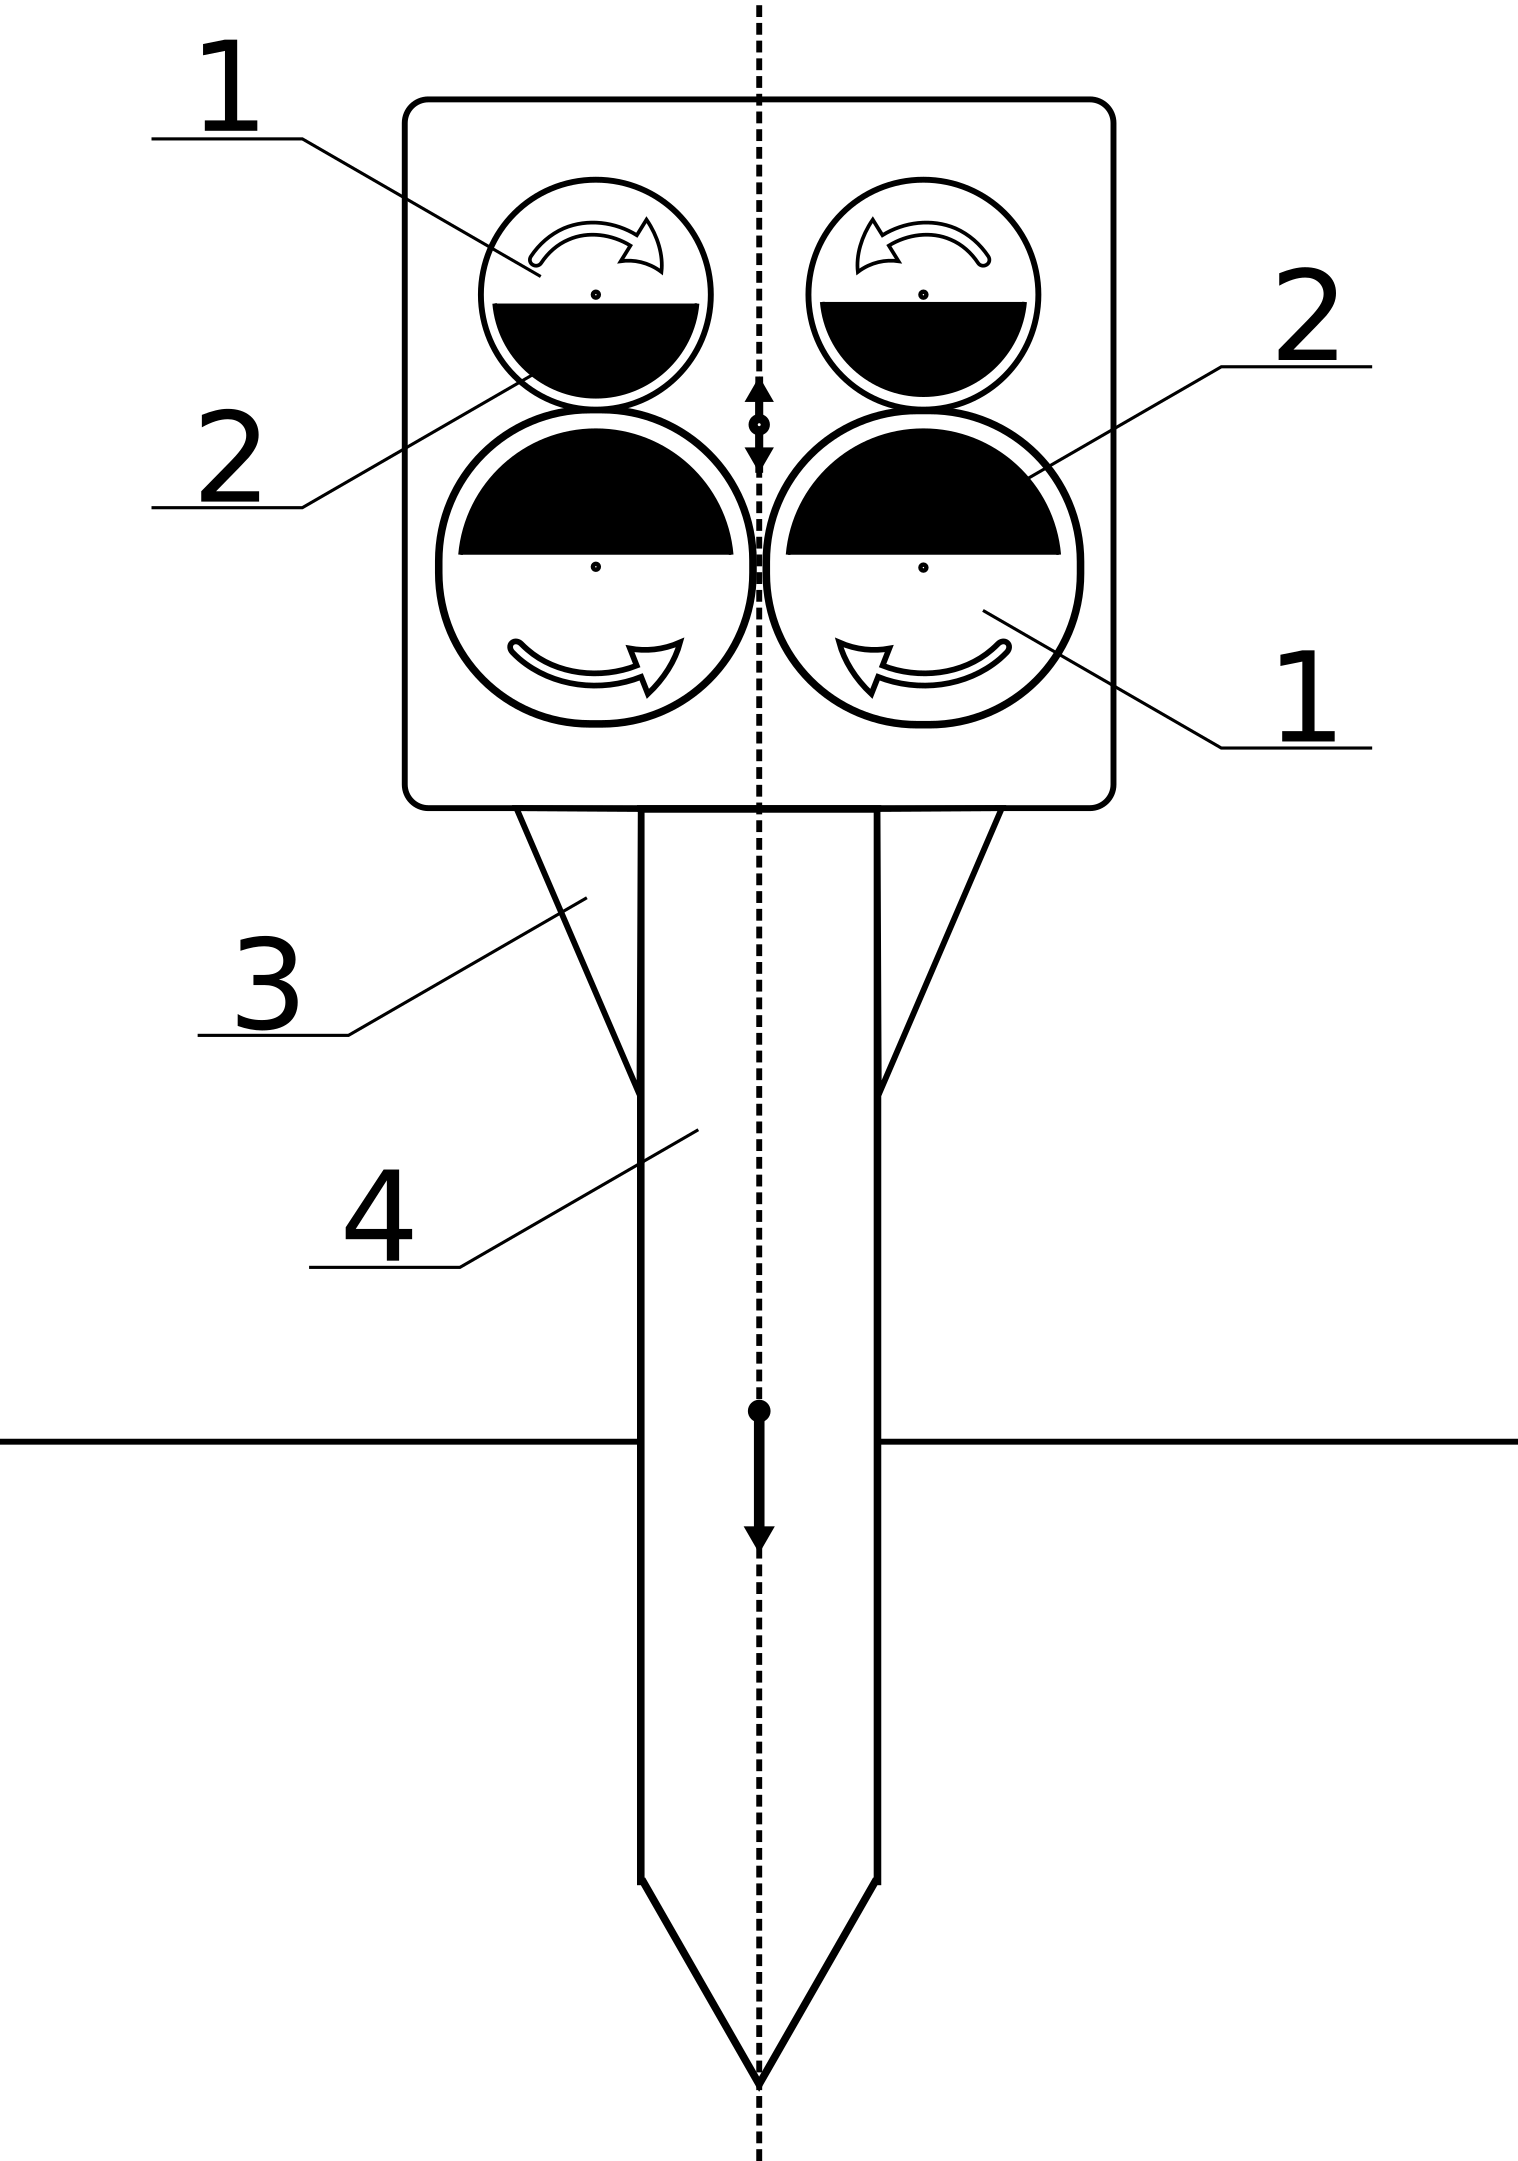
\includegraphics[width=1\linewidth]{../img/scheme_porg_2.png}
                        \caption{Схема вибрационного погружателя.}
                    \end{figure}
                \end{minipage}
            \end{minipage}
        \end{center}
    \end{frame}


    \begin{frame}
        \frametitle{Конструкция дебаланса}
        \begin{center}
            \begin{minipage}[h]{0.97\linewidth}
                \begin{minipage}[h]{0.6\linewidth}
                    Центробежная сила:
                    \begin{equation}
                        \begin{gathered}
                            F_{\textrm{центр.}} = m \cdot \omega^2 \cdot l \\
                            \textrm{где } l = \frac{4 r}{3 \pi}
                        \end{gathered}
                    \end{equation}
                    \\
                    Гармонические колебания:
                    \begin{equation}
                        \begin{gathered}
                            x(t) = \lambda \cos (\omega t) \\
                            \textrm{где } \lambda = m \cdot \omega^2 \cdot l
                        \end{gathered}
                    \end{equation}
                \end{minipage}
                \hfill
                \begin{minipage}[h]{0.36\linewidth}
                    \begin{figure}[h]
                        \centering
                        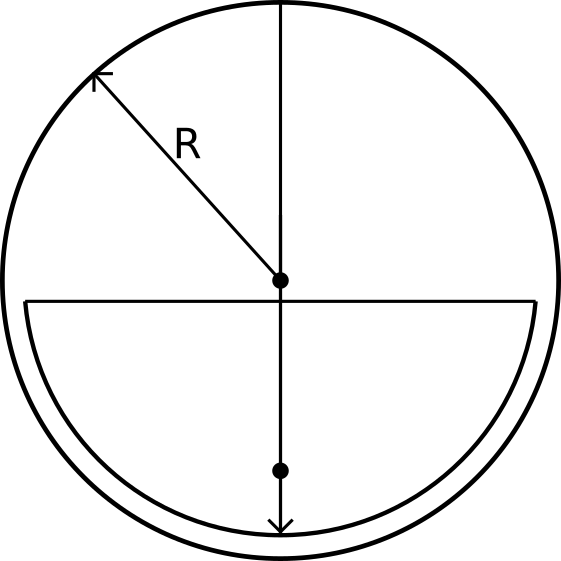
\includegraphics[width=1\linewidth]{../img/debalance.png}
                        \caption{Схема дебаланса.}
                    \end{figure}
                \end{minipage}
            \end{minipage}
        \end{center}
    \end{frame}


    \begin{frame}
        \frametitle{Конструкция пары дебалансов}
        \begin{center}
            \begin{minipage}[h]{0.97\linewidth}
                Гармонические колебания:
                \begin{equation}
                    \begin{gathered}
                        x(t) = 2 \lambda \cos (\omega t), \textrm{где } \lambda = m \cdot \omega^2 \cdot l
                    \end{gathered}
                \end{equation}
                Уравнение гармонического колебания для пары дебалансов в общем виде:
                \begin{equation}
                    \begin{aligned}
                        x(t) = 2 m_k \cdot (k \omega)^2 \cdot l(r_k) \cdot \cos (k \omega t)
                    \end{aligned}
                \end{equation}
                \begin{figure}[h]
                    \centering
                    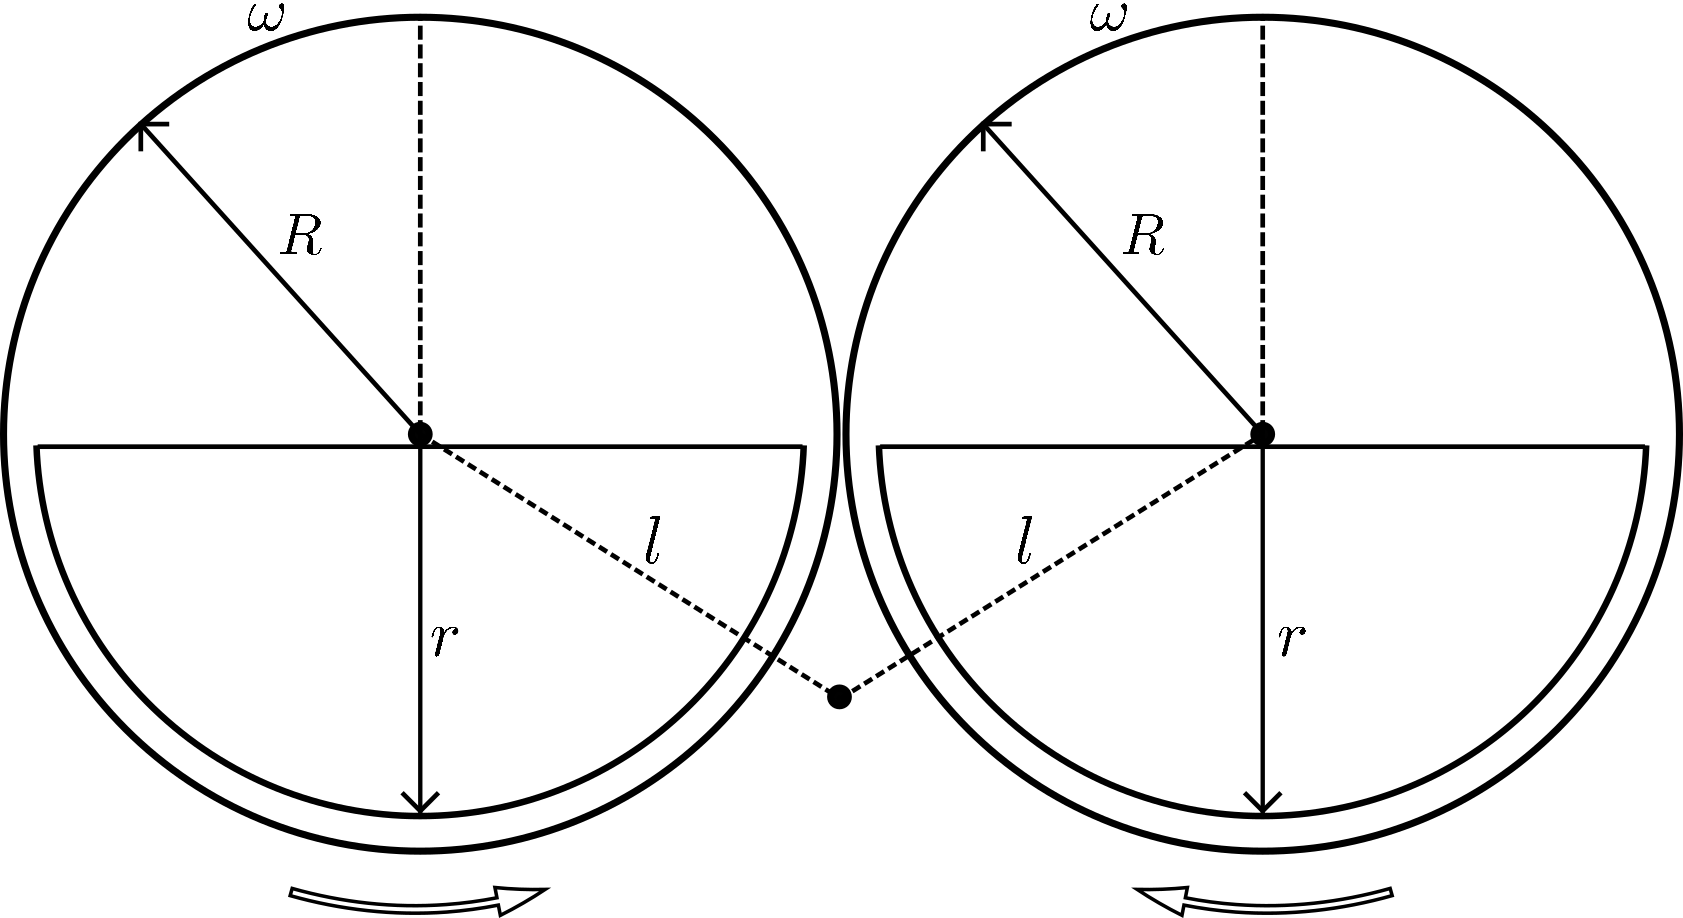
\includegraphics[width=0.52\linewidth]{../img/double_debalance.png}
                    \caption{Схема пары дебалансов.}
                \end{figure}
            \end{minipage}
        \end{center}
    \end{frame}


    \begin{frame}
        \frametitle{Гармонические колебания дебалансов}
        \begin{center}
            \begin{minipage}[h]{0.97\linewidth}
                Cумма гармонических колебаний для всех пар дебалансов:
                \begin{equation}\label{eq:harmonic_sum}
                    \begin{gathered}
                        F = \sum\limits_{k = 1}^n 2 \lambda_k \cdot \cos (k \omega t), \lambda = m \cdot \omega^2 \cdot l
                    \end{gathered}
                \end{equation}
                \begin{minipage}[h]{0.46\linewidth}
                    \begin{figure}[h]
                        \centering
                        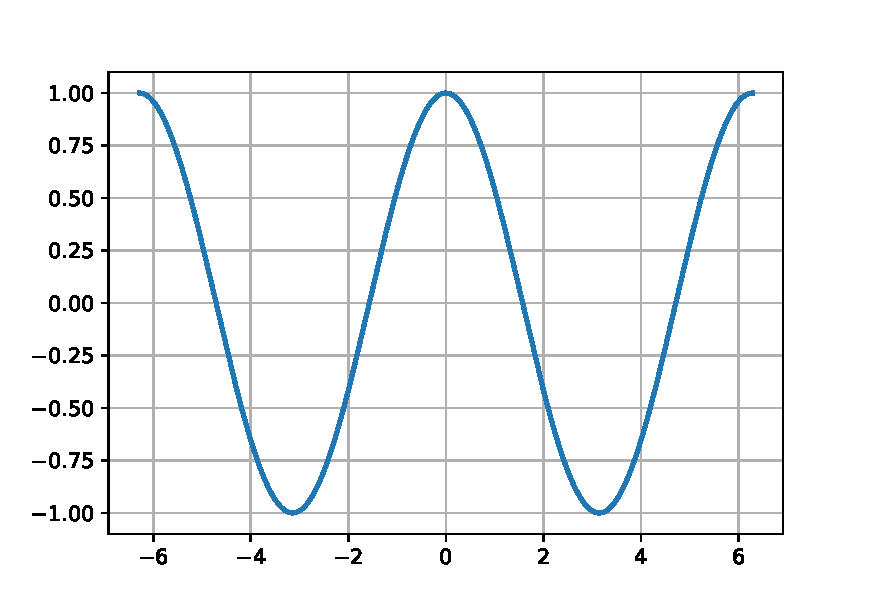
\includegraphics[width=1\linewidth]{../grap/impulse_1.pdf}
                        \caption{График работы выбропогружателя.}
                    \end{figure}
                \end{minipage}
                \hfill
                \begin{minipage}[h]{0.46\linewidth}
                    \begin{figure}[h]
                        \centering
                        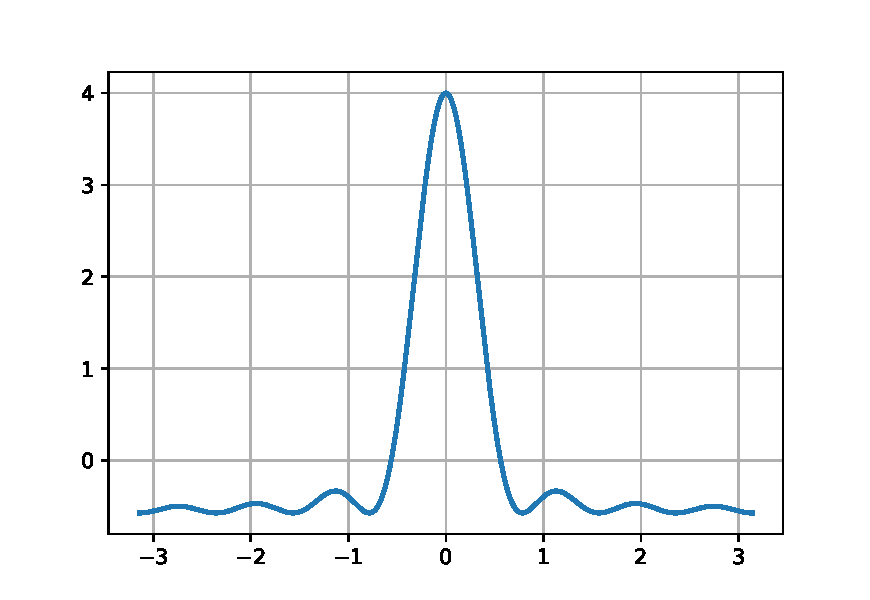
\includegraphics[width=1\linewidth]{../grap/impulse_7.pdf}
                        \caption{График работы импульсного погружателя.}
                    \end{figure}
                \end{minipage}
            \end{minipage}
        \end{center}
    \end{frame}


    \begin{frame}
        \frametitle{Задача оптимизации}
        \begin{center}
            \begin{minipage}[h]{0.97\linewidth}
                Пусть $f_{\max}(t)$ --- максимальное значение импульса силы за время $t$,
                $f_{\min}(t)$ --- минимальное значение импульса за время $t$. Тогда:
                \begin{equation}
                    \begin{gathered}
                        K = \left| \frac{f_{\max}(t)}{f_{\min}(t)} \right| \rightarrow \max
                    \end{gathered}
                \end{equation}

                Исходя из теоремы оптимальности модели полигармонического импульса многочлен (\ref{eq:harmonic_sum})
                является оптимальным тогда и только тогда, когда он с точностью до постоянного множителя имеет вид суммы Фейера:

                \begin{equation}\label{eq:feer}
                    \begin{gathered}
                        f_n(t) = \sum\limits_{k = 1}^n (n + 1 - k) \cos(kt)\\
                        \max \limits_{\lambda} K_n(\lambda) = n
                    \end{gathered}
                \end{equation}
                Из этого следует, что:
                \begin{equation}
                    \begin{gathered}
                        \lambda_k = \frac{n - k + 1}{n}
                    \end{gathered}
                \end{equation}
            \end{minipage}
        \end{center}
    \end{frame}


    \begin{frame}
        \begin{alertblock}{}
            \centerline{\large Спасибо за внимание!}
        \end{alertblock}
    \end{frame}
\end{document}
